\speaker{\Michel}

\begin{frame}
\frametitle{\underline{M}VC : Le modèle}
\begin{figure}[!h]
	\begin{center}
	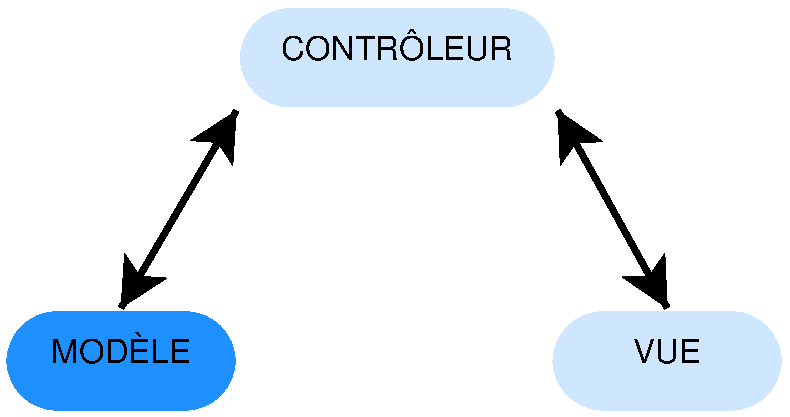
\includegraphics[scale=0.5]{images/mvcModele}
	\caption{Architecture \underline{M}VC}
	\end{center}
\end{figure}
Modèle :   cœur de l'application
\end{frame}

%%%%%%%%%%%%%%%%%%%%%%%%%%%%%%%%%%%%%%%%%%%%%%%%%%%

\begin{frame}
	\frametitle{\underline{M}VC : Le modèle}
	\begin{block}{Modélisation de la base de données}	
		\begin{itemize}
			\item Réalisation du diagramme de classe
			\item Création de la Base de Données et mapping avec les entités du projet
		\end{itemize}
	\end{block}
\end{frame}

%%%%%%%%%%%%%%%%%%%%%%%%%%%%%%%%%%%%%%%%%%%%%%%%%%%

\begin{frame}
	\frametitle{\underline{M}VC : Le modèle}
	
	\begin{block}{Création de la Base de Données et utilisation de l'ORM Doctrine}
		Deux approches possibles : 
		\begin{itemize}
			\item Top Down
				\begin{itemize}
					\item[$\rightarrow$] approche descendante
					\item[$\rightarrow$] système d'annotation dans les classes PHP
					\item[$\rightarrow$] génération des tables de la Base de Données
				\end{itemize}
			\item Buttom Up
				\begin{itemize}
					\item[$\rightarrow$] approche ascendante
					\item[$\rightarrow$] création de la Base de Données
					\item[$\rightarrow$] génération des fichiers de mapping et classes PHP
				\end{itemize}
		\end{itemize}
	\end{block} 

	
\end{frame}


%%%%%%%%%%%%%%%%%%%%%%%%%%%%%%%%%%%%%%%%%%%%%%%%%%%

\speaker{\Julie}
\begin{frame}
	\frametitle{\underline{M}VC : Le modèle}
	\begin{block}{Top Down}
		Avantages :
		\begin{itemize}
			\item Approche objet
			\item Doctrine initialement prévu pour une approche top down
		\end{itemize}
 
		Inconvénients :
		\begin{itemize}
			\item Non visibilité du cycle de vie
			\item Création d'une table intermédiaire pour les attributs multivalués
			\item Mauvaise gestion de l'héritage
			\item Mauvaise gestion des attributs d'association
			
		\end{itemize}
	\end{block}
\end{frame}

%%%%%%%%%%%%%%%%%%%%%%%%%%%%%%%%%%%%%%%%%%%%%%%%%%%

\begin{frame}
	\frametitle{\underline{M}VC : Le modèle}
	\begin{block}{Bottom up}
	Avantages :
		\begin{itemize}
			\item Propreté de la Base de Données
			\item Amélioration des performances
			\item Vérification des contraintes dans la Base de Données
		\end{itemize} 
	Inconvénients :
		\begin{itemize}
			\item ORM non adapté
			\item Vérification et modifications d'une partie des fichiers générés
		\end{itemize}
	\end{block}
  
\end{frame}

%%%%%%%%%%%%%%%%%%%%%%%%%%%%%%%%%%%%%%%%%%%%%%%%%%%

\begin{frame}
	\frametitle{\underline{M}VC : Le modèle}
	\begin{block}{Décision}
		\begin{itemize}
		\item Une bonne structure de base représente une anticipation des problèmes par la suite 
		\item Mieux adapté pour une possible utilisation au niveau Unicef France
		\end{itemize}
		
		
	\end{block}
\end{frame}